

\section*{K5/1. feladat: Hőterjedés sík kazánfalban}
\addcontentsline{toc}{section}{K5/1. feladat: Hőterjedés sík kazánfalban}

\begin{tabular}{ | p{2cm} | p{14cm} | } 
	\hline
	Név & Szalay István \\ 
	\hline
	Szak & \\ 
	\hline
	Félév & 2019/2020 II. (tavaszi) félév \\ 
	\hline
\end{tabular}
\vspace{0.5cm}

\noindent Egy kazánban \SI{10}{\bar} nyomású gőzt termelnek. A kazánfal belső felülete \SI{200}{\celsius}, külső (tűztér felőli) felülete pedig \SI{395}{\celsius} hőmérsékletű. A kazán fala $\delta_1 = \SI{16}{\milli\meter}$ vastagságú.

\vspace{2mm}
\noindent  A kazán falának hővezetési tényezője $\lambda_1 = \SI{43}{\watt\per\meter\kelvin}$. (A kazán falát síkfalnak tekintjük.)

\begin{figure}[h]
	\centering
	\begin{subfigure}[b]{0.33\textwidth} 
		\centering
		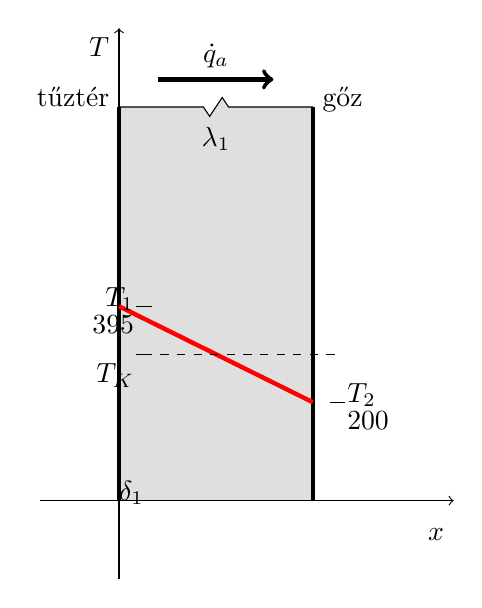
\begin{tikzpicture}
			\pgfmathsetmacro{\d}{16/6.5}
			\pgfmathsetmacro{\L}{5}
			\pgfmathsetmacro{\TA}{395/160}
			\pgfmathsetmacro{\TB}{200/160}
			\pgfmathsetmacro{\TK}{(\TA+\TB)/2}
			
			% Fal
			\fill[gray,opacity=0.25] (0,0) -- (0,\L) -- ({\d/2-0.16},\L) -- ({\d/2-0.08}, {\L-0.12}) -- ({\d/2+0.08}, {\L +0.12}) -- ({\d/2+0.16}, \L) -- (\d, \L) -- (\d, 0);
			\draw[] (0,\L) -- ({\d/2-0.16},\L) -- ({\d/2-0.08}, {\L-0.12}) -- ({\d/2+0.08}, {\L+0.12}) -- ({\d/2+0.16}, \L) -- (\d, \L);
			\draw[ultra thick] (0,0) -- (0,\L);
			\draw[ultra thick] (\d, 0) -- (\d, \L);
			
			% Feliratok
			\node[anchor=base east] at (0, \L) {tűztér};
			\node[anchor=base west] at (\d, \L) {gőz};
			
			% Tengelyek
			\draw[->] (0,-1) -- (0,\L+1) node[anchor=north east]{$T$};
			\draw[->] (-1,0) -- (4.25,0) node[anchor=base east, shift={(0,-0.5)}]{$x$};
			
			% Hőáram és hőáramsűrűség
			\draw[->, ultra thick] (0.5,{\L+0.35}) -- ({\d/2},{\L+0.35}) node[anchor=south]{$\dot{q}_a$} -- ({\d - 0.5},{\L+0.35});
			
			% A hővezetési tényező
			\node[anchor=base] at ({\d/2},{\L-0.5}) {$\lambda_1$};
			
			% T(x)
			\draw[red, ultra thick] (0,\TA) -- (\d,\TB);
			
			% A delta_1 falvastagság
			\pgflength[xa=0, ya=0, xb=\d, yb=0, alim=0]{$\delta_1$};
			
			% A hőmérséklet értékek
			\draw (-0.1,\TA) -- (0.1,\TA);
			\node[anchor=base east] at (0,\TA) {$T_1$};
			\node[anchor=north east] at (0,\TA) {$\SI{395}{\celsius}$};
			
			\draw (-0.1+\d,\TB) -- (0.1+\d,\TB);
			\node[anchor=base west] at (\d,\TB) {$T_2$};
			\node[anchor=north west] at (\d,\TB) {$\SI{200}{\celsius}$};
			
			% A közepes hőmérséklet
			\draw[dashed] (0,\TK) -- (\d,\TK);
			\draw (-0.1,\TK) -- (0.1,\TK);
			\node[anchor=north east] at (0,\TK) {$T_K$};
			
		\end{tikzpicture}
		\caption{A hőmérséklet-hely függvény az a) esetben.}
	\end{subfigure}
	\begin{subfigure}[b]{0.31\textwidth}
		\centering
		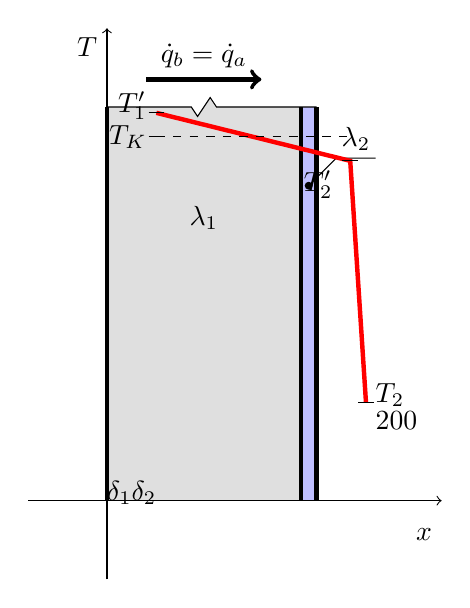
\begin{tikzpicture}
			\pgfmathsetmacro{\d}{16/6.5}
			\pgfmathsetmacro{\v}{1.2/6}
			\pgfmathsetmacro{\L}{5}
			\pgfmathsetmacro{\TA}{788/160}
			\pgfmathsetmacro{\TB}{690.5/160}
			\pgfmathsetmacro{\TC}{200/160}
			\pgfmathsetmacro{\TK}{(\TA+\TB)/2}
			
			% Fal
			\fill[gray,opacity=0.25] (0,0) -- (0,\L) -- ({\d/2-0.16},\L) -- ({\d/2-0.08}, {\L-0.12}) -- ({\d/2+0.08}, {\L +0.12}) -- ({\d/2+0.16}, \L) -- (\d, \L) -- (\d, 0);
			\fill[blue,opacity=0.25] (\d, \L) -- (\d, 0) -- (\d+\v, 0) -- (\d+\v, \L);
			\draw[] (0,\L) -- ({\d/2-0.16},\L) -- ({\d/2-0.08}, {\L-0.12}) -- ({\d/2+0.08}, {\L+0.12}) -- ({\d/2+0.16}, \L) -- (\d, \L) -- (\d+\v, \L);
			\draw[ultra thick] (0,0) -- (0,\L);
			\draw[ultra thick] (\d, 0) -- (\d, \L);
			\draw[ultra thick] (\d+\v, 0) -- (\d+\v, \L);
			
			% Tengelyek
			\draw[->] (0,-1) -- (0,\L+1) node[anchor=north east]{$T$};
			\draw[->] (-1,0) -- (4.25,0) node[anchor=base east, shift={(0,-0.5)}]{$x$};
			
			% Hőáram és hőáramsűrűség
			\draw[->, ultra thick] (0.5,{\L+0.35}) -- ({\d/2},{\L+0.35}) node[anchor=south]{$\dot{q}_b = \dot{q}_a$} -- ({\d - 0.5},{\L+0.35});
			
			% A hővezetési tényező
			\node[anchor=base] at ({\d/2},{\L-1.5}) {$\lambda_1$};
			\node[anchor=base] at ({\d+\v+0.5},{\L-0.5}) {$\lambda_2$};
			\draw ({\d+\v+0.75},{\L-0.65}) -- ({\d+\v+0.25},{\L-0.65}) -- ({\d+\v/2},{\L-1});
			\fill[] ({\d+\v/2},{\L-1}) circle[radius=0.05];
			
			% A falvastagságok
			\pgflength[xa=0, ya=0, xb=\d, yb=0, alim=0]{$\delta_1$};
			\pgflength[xa=\d, ya=0, xb=\d+\v, yb=0, alim=0, a=0, belül=2]{$\delta_2$};
			
			% T(x)
			\draw[red, ultra thick] (0,\TA) -- (\d,\TB) -- (\d+\v,\TC);
			
			% Falhőmérsékletek
			\draw (-0.1,\TA) -- (0.1,\TA);
			\node[anchor=base east] at (0,\TA) {$T_1'$};
			
			\draw (-0.1+\d,\TB) -- (0.1+\d,\TB);
			\node[anchor=north east] at (\d-0.1,\TB) {$T_2'$};
			
			\draw (-0.1+\d+\v,\TC) -- (0.1+\d+\v,\TC);
			\node[anchor=base west] at (\d+\v,\TC) {$T_2$};
			\node[anchor=north west] at (\d+\v,\TC) {$\SI{200}{\celsius}$};
			
			% A közepes hőmérséklet
			\draw[dashed] (0,\TK) -- (\d,\TK);
			\draw (-0.1,\TK) -- (0.1,\TK);
			\node[anchor=east] at (0,\TK) {$T_K$};
			
		\end{tikzpicture}
		\caption{A hőmérséklet-hely függvény az b) esetben.}
	\end{subfigure}
	\begin{subfigure}[b]{0.31\textwidth}
		\centering
		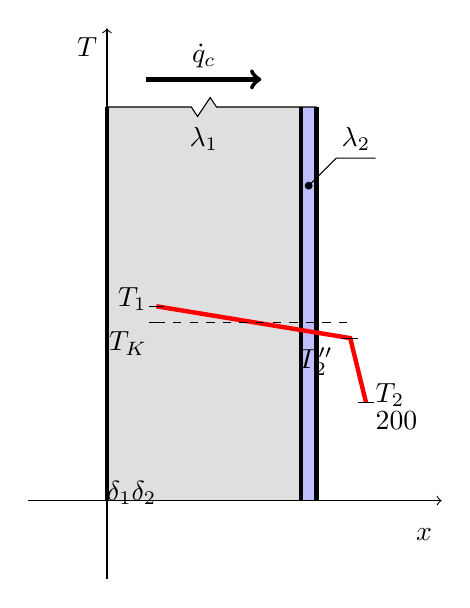
\begin{tikzpicture}
			\pgfmathsetmacro{\d}{16/6.5}
			\pgfmathsetmacro{\v}{1.2/6}
			\pgfmathsetmacro{\L}{5}
			\pgfmathsetmacro{\TA}{395/160}
			\pgfmathsetmacro{\TB}{330.3/160}
			\pgfmathsetmacro{\TC}{200/160}
			\pgfmathsetmacro{\TK}{(\TA+\TB)/2}
			
			% Fal
			\fill[gray,opacity=0.25] (0,0) -- (0,\L) -- ({\d/2-0.16},\L) -- ({\d/2-0.08}, {\L-0.12}) -- ({\d/2+0.08}, {\L +0.12}) -- ({\d/2+0.16}, \L) -- (\d, \L) -- (\d, 0);
			\fill[blue,opacity=0.25] (\d, \L) -- (\d, 0) -- (\d+\v, 0) -- (\d+\v, \L);
			\draw[] (0,\L) -- ({\d/2-0.16},\L) -- ({\d/2-0.08}, {\L-0.12}) -- ({\d/2+0.08}, {\L+0.12}) -- ({\d/2+0.16}, \L) -- (\d, \L) -- (\d+\v, \L);
			\draw[ultra thick] (0,0) -- (0,\L);
			\draw[ultra thick] (\d, 0) -- (\d, \L);
			\draw[ultra thick] (\d+\v, 0) -- (\d+\v, \L);
			
			% Tengelyek
			\draw[->] (0,-1) -- (0,\L+1) node[anchor=north east]{$T$};
			\draw[->] (-1,0) -- (4.25,0) node[anchor=base east, shift={(0,-0.5)}]{$x$};
			
			% Hőáram és hőáramsűrűség
			\draw[->, ultra thick] (0.5,{\L+0.35}) -- ({\d/2},{\L+0.35}) node[anchor=south]{$\dot{q}_c$} -- ({\d - 0.5},{\L+0.35});
			
			% A hővezetési tényező
			\node[anchor=base] at ({\d/2},{\L-0.5}) {$\lambda_1$};
			\node[anchor=base] at ({\d+\v+0.5},{\L-0.5}) {$\lambda_2$};
			\draw ({\d+\v+0.75},{\L-0.65}) -- ({\d+\v+0.25},{\L-0.65}) -- ({\d+\v/2},{\L-1});
			\fill[] ({\d+\v/2},{\L-1}) circle[radius=0.05];
			
			% A falvastagságok
			\pgflength[xa=0, ya=0, xb=\d, yb=0, alim=0]{$\delta_1$};
			\pgflength[xa=\d, ya=0, xb=\d+\v, yb=0, alim=0, a=0, belül=2]{$\delta_2$};
			
			% T(x)
			\draw[red, ultra thick] (0,\TA) -- (\d,\TB) -- (\d+\v,\TC);
			
			% Falhőmérsékletek
			\draw (-0.1,\TA) -- (0.1,\TA);
			\node[anchor=base east] at (0,\TA) {$T_1$};
			%\node[anchor=north east] at (0,\TA) {$\SI{395}{\celsius}$};
			
			\draw (-0.1+\d,\TB) -- (0.1+\d,\TB);
			\node[anchor=north east] at (\d-0.1,\TB) {$T_2''$};
			
			\draw (-0.1+\d+\v,\TC) -- (0.1+\d+\v,\TC);
			\node[anchor=base west] at (\d+\v,\TC) {$T_2$};
			\node[anchor=north west] at (\d+\v,\TC) {$\SI{200}{\celsius}$};
			
			% A közepes hőmérséklet
			\draw[dashed] (0,\TK) -- (\d,\TK);
			\draw (-0.1,\TK) -- (0.1,\TK);
			\node[anchor=north east] at (0,\TK) {$T_K$};
			
		\end{tikzpicture}
		\caption{A hőmérséklet-hely függvény a c) esetben.}
	\end{subfigure}
\end{figure}

\subsubsection*{a) Határozzuk meg a fal közepes hőmérsékletét és a falban kialakuló hőáramsűrűséget!}

A fal közepes hőmérséklete a lineáris hőmérsékleteloszlás miatt a falhőmérsékletek átlaga:
\begin{equation}
	T_K = \frac{T_1 + T_2}{2} = \SI{297.5}{\celsius}
\end{equation}

Nem lineáris hőmérsékleteloszlás esetén a hőmérséklet-hely függvény határozott integráljának és a falvastagságnak a hányadosa a közepes hőmérséklet.

A hőáramsűrűség a falban
\begin{equation}
	\dot{q}_a = \frac{\lambda_1}{\delta_1} (T_1 - T_2) = \SI{524}{\kilo\watt\per\meter\squared}
\end{equation}
Ebben a feladatban a kazánfal oldalain végbemenő hőátadást tökéletesnek tekintjük, azaz a falhőmérsékletek megegyeznek a közeghőmérsékletekkel.

\subsubsection*{b) A kazán falára $\delta_2 = \SI{1.2}{\milli\meter}$ vastag kazánkőréteg rakódik. Változatlan gőztermelés és gőznyomás esetén számítsuk ki a kazán falának közepes hőmérsékletét!}

A vízkőréteg hővezetési tényezője $\lambda_2 = \SI{1.6}{\watt\per\meter\kelvin}$.

\vspace{2mm}

A "változatlan gőztermelés" kifejezés azt jelenti, hogy a gőzoldali falhőmérséklet és a hőáramsűrűség a falban nem változik. A vízkőréteg miatt a hőáramsűrűség csak úgy maradhat azonos $\dot{q}_a$-val, hogy a tűztér oldali $T_1'$ falhőmérséklet sokkal nagyobb $T_1$-nél, a $T_2'$ falhőmérséklet pedig nem azonos a gőzoldali $T_2$ hőmérséklettel. A vízkőréteg hővezetési tényezője sokkal kisebb a kazánlemezénél, ezért a kisebb rétegvastagság ellenére nagyobb hőmérséklet esik rajta.

A fal közepes hőmérséklete itt is a két falhőmérséklet átlaga:
\begin{equation}
	T_K' = \frac{T_1' + T_2'}{2}
\end{equation}

A $T_1'$ és a $T_2'$ falhőmérséklet a $q_b$ hőáramsűrűség alapján számítható ki:
\begin{equation}
	\dot{q}_b = \dot{q}_a = \frac{\lambda_1}{\delta_1} (T_1' - T_2') = \frac{\lambda_2}{\delta_2} (T_2' - T_2)
\end{equation}

\begin{equation}
	T_2' = T_2 + \frac{\delta_2}{\lambda_2}\dot{q}_a = \SI{200}{\celsius} + \frac{\SI{1.2}{\milli\meter}}{\SI{1.6}{\watt\per\meter\kelvin}} \SI{524}{\kilo\watt\per\meter\squared} = \SI{593}{\celsius}
\end{equation}

\begin{equation}
	T_1' = T_2' + \frac{\delta_1}{\lambda_1}\dot{q}_a = \SI{593}{\celsius} + \frac{\SI{16}{\milli\meter}}{\SI{43}{\watt\per\meter\kelvin}} \SI{524}{\kilo\watt\per\meter\squared} = \SI{788}{\celsius}
\end{equation}

\subsubsection*{c) Ha szilárdsági okok miatt a fal hőmérséklete nem emelkedhet, de a gőznyomás változatlan, mekkora lesz a hőáramsűrűség?}

Ha gőznyomás nem változik, akkor a gőz hőmérséklete sem változik, mivel a kazánban a nedves gőzmezőbe eső állapotú a víz, és ott T--s diagram szerint az izotermák és az izobár vonalak egybeesnek. Tehát a gőzoldali hőmérséklet $T_2$. Ha szilárdsági okok miatt a fal hőmérséklete nem emelkedhet, akkor a tűztér oldali hőmérséklet az eredeti $T_1$.

A $\dot{q}_c$ hőáramsűrűség azonos a kazánfalban és a vízkőrétegben:
\begin{equation}
	\dot{q}_c = \frac{\lambda_1}{\delta_1} (T_1 - T_2'') = \frac{\lambda_2}{\delta_2} (T_2'' - T_2)
\end{equation}

Kifejezve a két hőmérsékletkülönbséget, és összeadva a két egyenletet:
\begin{equation}
	\left.
	\begin{array}{lcl}
		\dot{q}_c \dfrac{\delta_1}{\lambda_1} = (T_1 - T_2'') \\
		\dot{q}_c \dfrac{\delta_2}{\lambda_2} = (T_2'' - T_2)
	\end{array}
	\right\rbrace
	\quad \Rightarrow \quad 
	\dot{q}_c \left(\dfrac{\delta_1}{\lambda_1} + \dfrac{\delta_2}{\lambda_2} \right) = (T_1 - T_2) 
	\quad \Rightarrow \quad 
	\dot{q}_c = 
	\SI{173.78}{\kilo\watt\per\meter\squared}
\end{equation}

A fenti két egyenletet kétismeretlenes egyenletrendszernek is tekinthetjük, ahol a hőáramsűrűség mellett a másik ismeretlen a $T_2''$ falhőmérséklet. A hőáramsűrűséget visszahelyettesítve megkaphatjuk az értékét:
\begin{equation}
	T_2'' = T_1 - \dot{q}_c \dfrac{\delta_1}{\lambda_1} = \SI{330.34}{\celsius}
\end{equation}

\pagebreak
